\chapter{Background Details}

This chapter provides insights about multiple areas related to Federated Meta-Learning. It takes a deeper look into the fundamental concepts related to this research and also discusses other related work and existing research in the fields of Meta-Learning, Algorithm Selection and Automated Machine Learning.

\section{Meta-Learning}
Meta-Learning in the context of Machine Learning is learning how to learn. It can also be attributed to the study of principal methods that use meta-knowledge to create efficient models by using machine learning techniques. Meta-Learning algorithm use experience to learn how to perform a certain task, these modified learner are better than the original learner as they have gained additional experience. Each algorithm works on a set of assumptions about the data, that it is \textbf{inductively biased}, meaning that the algorithm will learn well (or work as expected) given that the bias matches the learning problem at hand. This introduces restrictions about the type of data and the techniques used to collect this data to perform the meta-learning. By using different types of meta-data, like in this case meta-features of the dataset, it is possible to learn to effectively solve a learning problem. There are three approaches to meta-learning algorithm model-based, metrics-based and optimisation-based.

\begin{itemize}
    \item \textbf{Model-Based}:
    This type of meta-learning models updates its model-parameters rapidly with training over a dataset.
    \item \textbf{Metric-Based}:
    The core idea in type of models is similar to that of nearest neighbours algorithms and a relationship between tasks are established.
    \item \textbf{Optimization-Based}:
    In this case the algorithms plays around with the optimisation algorithms which is used to train the model.
\end{itemize}

\section{Automated Machine Learning}
Automated Machine Learning or AutoML, is the process of automating the time consuming task of Algorithm Selection and Optimizing the Hyper-Parameters. Traditional machine learning model creation is highly resource-intensive and requires significant domain knowledge and time to create and compare dozens of models. With AutoML, we will be able to accelerate the time it takes to get ML models with great ease and efficiency. There are many tools that offer to perform this complicated and time consuming task like Auto-Sklearn, Auto-Weka, Auto-Keras, etc. Apart from these tasks AutoML tools also perform feature selection, featuring engineering, data pre-processing and also analyse and tune the results. Among the various tasks performed by the AutoML Tools, the tasks that consume the most of the time are Algorithm Selection and Hpyer-Parameter Optimisation. 

\subsection{Algorithm Selection}
Algorithm Selection is usually done on an instance by instance basis, meaning different algorithm have to be chosen for different datasets. An algorithm which performs exceptionally well for one dataset may perform poorly for another. The task of choosing an algorithm is dependent on what data we have and how we choose to use it, meaning how the data is cleaned, encoded, imputed, distributed and also how they co-relate with other features or variables within the dataset. The manual task of algorithm selection involves studying and understanding the relationship between different features of the dataset, trying various types of pre-processing steps to bring out the inter-feature relationship which best explains the data. 

The tools which perform Algorithm Selection choose the best performing algorithm by predicting the performance of each algorithm for a given task by running various algorithms on a subset of the entire dataset repeatedly after performing different pre-processing steps and then choose the best performing algorithm on that subset for the task. Though this is just a over-simplified explanation of what the libraries do internally, this task is more of a straight forward approach which reduces the effort that a developer need to put in to select an algorithm. But this process comes with a huge trade-off, it takes up a lot of time, electricity and computational power before it could suggest the best suited algorithm for the task. Even if the task is to find the best algorithm for a previously seen dataset the entire process is repeated.

\subsection{Algorithm Configuration}

The task of Algorithm Configuration can be attributed to Hyper-Parameter Optimisation / Tuning, which is a process of selecting a set of optimal parameters for an algorithm for which it performs best on a dataset. A hyper-parameter is a parameter whose value is used control how a machine learning algorithm solves or learns to solve a given problem. Hyper-Parameter Optimisation of an Algorithm is a type of Optimisation problem. And a typical Optimisation problem consists of minimising or maximizing the set of parameters along with the metric. This task takes an expert with an in-depth domain knowledge a lot of time to solve, and is not something that can be performed with ease by a developer and hence the alternate approach of automating the task.

There are various optimisation strategies, among them, the commonly used strategies are: Grid search, Random search, Hill Climbing and Bayesian optimization. These techniques are used in combination with cross-validation for evaluating how the results of a statistical analysis will generalise irrespective of the dataset. The working of these strategies are out of scope of this paper, but to give an brief understanding, Grid search is a hyper-parameter tuning approach that will build and evaluate various models, where each model is build on a combination of algorithm parameters specified in a grid. But the important thing to note is that these strategies takes up a great deal of time, electricity and computational power, before a optimal set of hyper-parameter can be chosen for an algorithm-dataset pair.

\section{Workflow of AutoML Libraries}
\label{workflow-automl}

In this section we will discuss about the workflow of AutoML libraries without getting to the details regarding the internal workings of the algorithms or the libraries. The figure \ref{automl-workflow-diagram} represents the workflow of a typical AutoML project for a given task or dataset. The data is split into training and testing datasets, the training dataset is first sent to the library for the purpose of model creation. Here, the dataset is pre-processed using various techniques like data-cleaning, data imputation, data encoding, feature selection, feature exploration, feature engineering, feature co-relation, etc..

\begin{figure}[t]
    \centering
    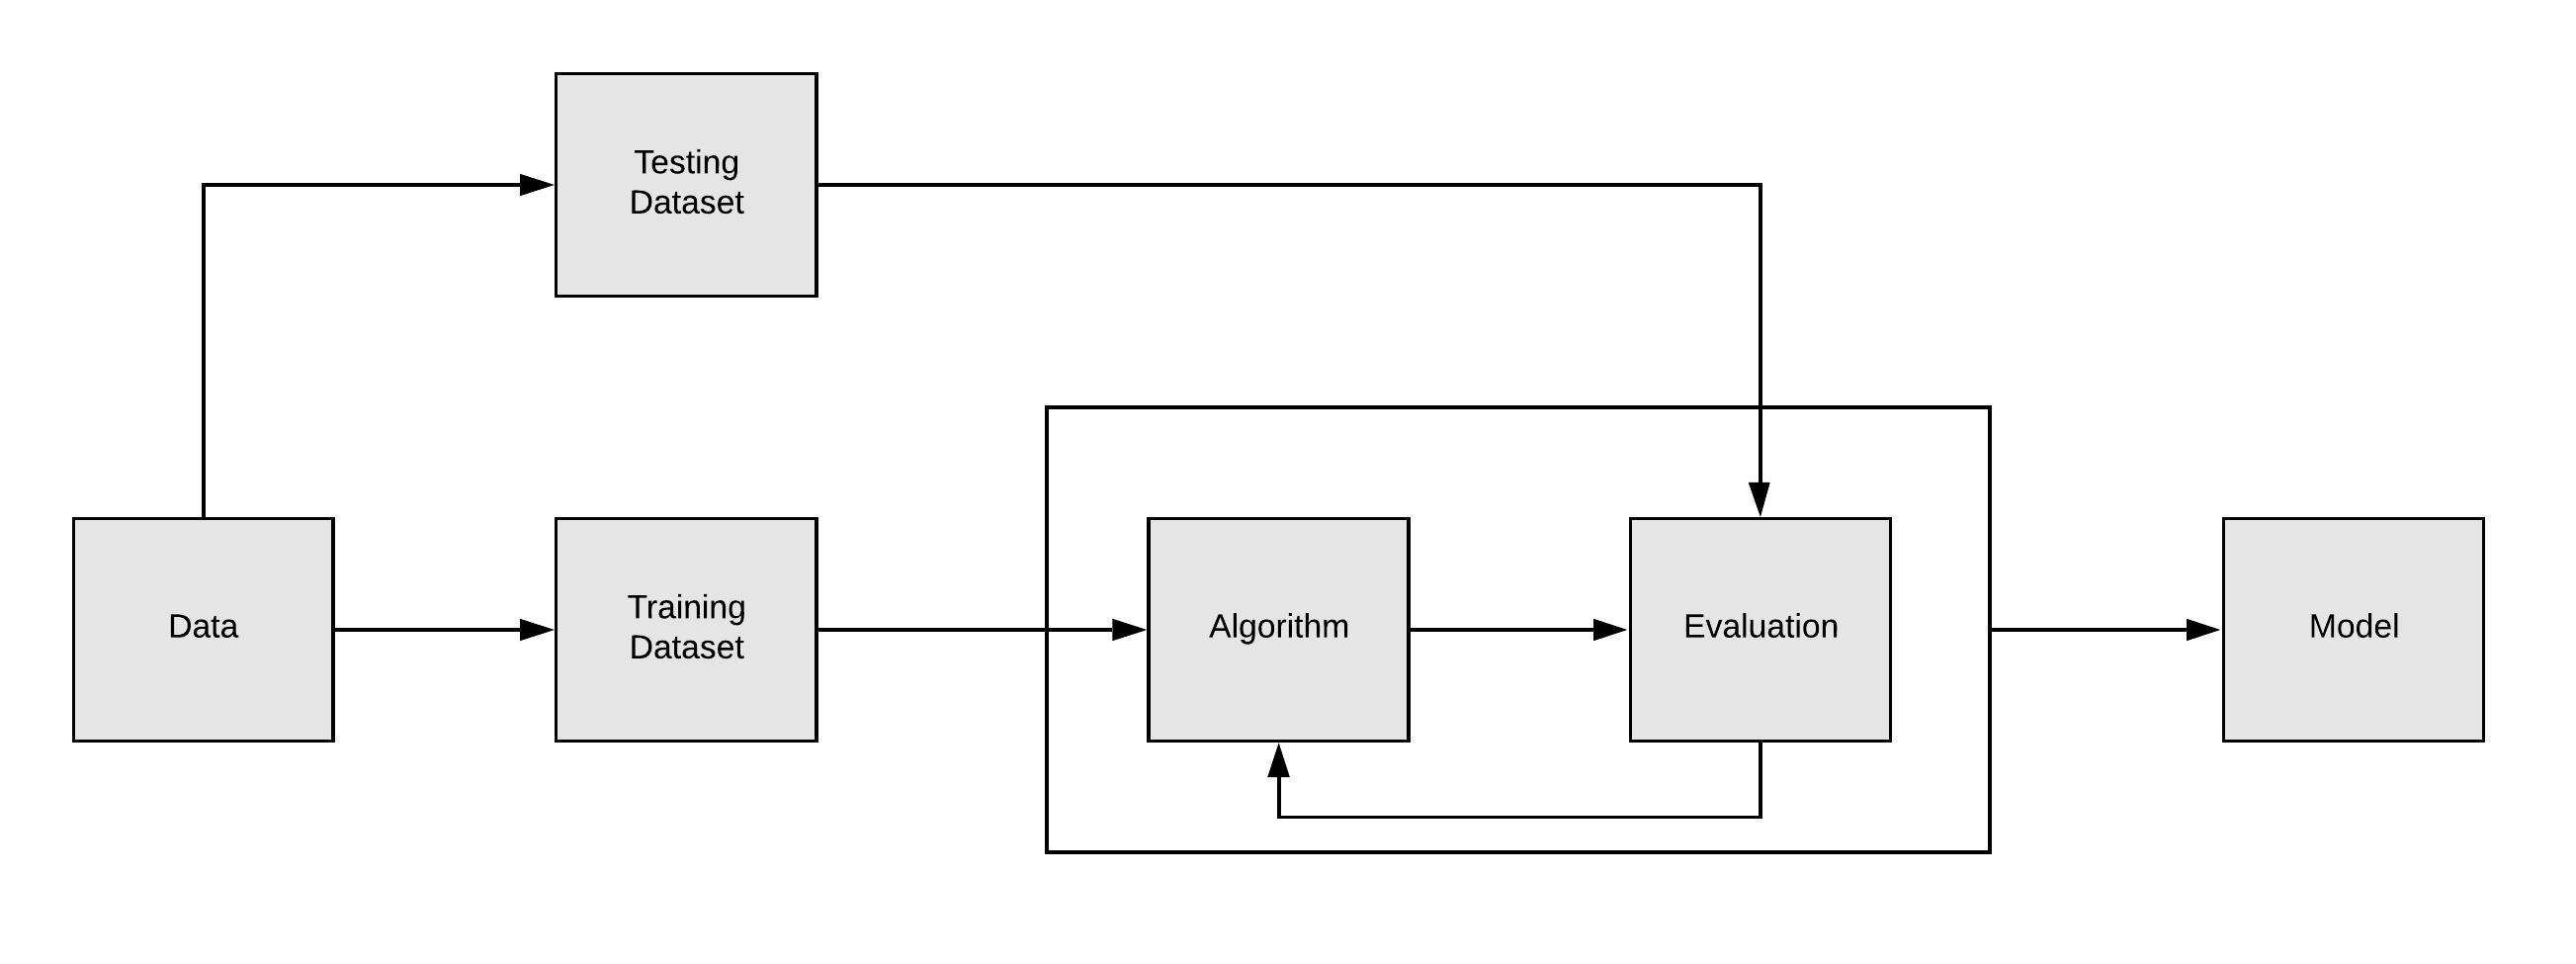
\includegraphics[width=16cm]{images/ML Workflow.jpeg}
    \caption{AutoML Workflow Diagram}
    \label{automl-workflow-diagram}
\end{figure}

Once, the data has been pre-processed, the dataset is split into a smaller subsets of the training dataset. One such subset is randomly chosen on which multiple algorithms are run to train and create a model for comparison and evaluation. Once the training and model creation of all chosen algorithms are completed, these models are evaluated based on multiple parameters one of which is their performance of an unseen data. When the performance metrics are calculated these models are evaluated and compared between each other and the best performing model is chosen for further training. Depending on the internal evaluation strategy of the AutoML tool used, more than one algorithm can be chosen for further training. Once these model(s) are chosen they are trained on various configurations of hyper-parameters using one of these search strategies; Grid Search, Randomized Search, Bayesian Optimization, etc. Once these models are trained and there hyper-parameters are optimised on the complete training dataset, they are evaluated against the testing dataset and the final best performing model is returned to the user.

%% a multi-line comment as an if statement
\if false

\section{Project Overview}
To tackle this repetitive and time consuming nature of these task, Dr. Joeran Beel proposed, what he called Federated Meta-Learning. Applying the concept of Federated Meta Learning, I have build an application called FMLearn to implement the same. Before explaining what the application is and what is does, some important information of this application are as follows. FMLearn is an application developed using the client-server model, which allows the exchange of meta-data about machine learning models and data for the purpose of meta-learned algorithm selection and configuration. In this Client-Server architecture the Client here is a popular Machine Learning package called Scikit-Learn which has been modified to the needs of the project. The client also enlists the help of another popular AutoML package for meta-data collection called Auto-Sklearn. 

\subsection{The Client: Scikit-Learn}
The client performs 2 crucial roles, one is to publish / send data to the server, which is then used by FMLearn to learn from and use this knowledge to make future predictions for tasks. The other task is to retrieve data from FMLearn, the data consists of Algorithm Predictions for previously seen or unseen datasets. The ideal choice for a client in such a role would be any popular and easy to use Machine Learning Library, and my choice was to use Scikit-Learn.

Scikit-learn \citep{scikit-learn} is a widely used, free and open source machine learning library\footnote{https://pypi.org/project/scikit-learn/}. I have used this as the client in the client-server model of my project to collect the information regarding how different classification, regression and clustering algorithms perform on various datasets and then publish / send this information about the model and other meta-data collected to the server - FMLearn - via the API endpoints which are made publicly available. It  also performs the role of retrieving the predicted algorithm for a previously seen or unseen task from the server via other exposed API's.

\subsection{The Server: FMLearn}
The server is a Python Application, which serves API's requests providing the caller with the requested details. It also acts as a knowledge base for all the data that is collected using the client, and learns from this knowledge base and suggests algorithms for a given task. It also has a very minimal user interface which explains the applications and provides links to various other useful information which might be required for the user.

\subsection{Meta-Features from Auto-Sklearn}
The tasks or datasets on which these algorithms run on are described by their meta-features which are obtained using the Auto-sklearn \citep{feurer:m} library via the client and this information about the meta-data about the data along with performance details of the algorithm on a particular task is sent / published to the server via an API call.

\fi

\section{Meta-Features}
\label{meta-feat-realted-work}
In the notion of Meta-Learning (MtL), Meta-Features are measures used to describe datasets and their relationship with algorithm bias. Meta-Features are used in Meta-Learning and AutoML tasks to describe the underlying dataset to create a machine learning, recommender systems and other models. The Meta-Features can be categorised to various groups, namely: General, Statistical, Information-theoretic, Model-based, landmarking, Relative Landmarking, Clustering, Complexity, etc. \citep{meta-features-1} \citep{meta-features-2} \citep{meta-features-3}. The most frequently adopted meta-features in three of the important categories used in this research are:
\begin{itemize}
    \item \textbf{General Meta-features}:
    Number of observations, Number of attributes, Number of output values, Dataset dimensionality.
    
    \item \textbf{Statistical Meta-features}:
    Standard deviation, Coefficient of variation, Covariance, Linear correlation coefficient, Skewness, Kurtosis
    
    \item \textbf{Information-Theoretic Meta-features}:
    Normalized class entropy, Normalized attribute entropy, Joint entropy of class and attribute, Mutual information of class and attribute, Equivalent number of attributes, Noise-signal ratio.
\end{itemize}

The Meta-Features discussed above are just a small sample of various possible characterisation features \citep{meta-features-1} \citep{meta-features-2} \citep{meta-features-3} , this is not an exhaustive list and details about these features are out of scope of this research.

\section{Related Work}

\subsection*{Algorithm Selection}

The field of algorithm selection and configuration is an area of intense research, according to Wikipedia, as stated by Rice in \citep{rice197665}, the process of algorithm selection is defined as:

\par\noindent\rule{\textwidth}{0.4pt}\newline
\textbf{Definition 1:} Given a portfolio ${\displaystyle{\mathcal{P}}}$ of algorithms ${\displaystyle{\mathcal{A}} \in {\mathcal{P}}}$, a set of instances ${\displaystyle{i \in {\mathcal{I}}}}$ and a cost metric ${\displaystyle{m:{\mathcal{P}} \times {\mathcal{I}} \to \mathcal{R}}}$, the algorithm selection problem consists of finding a mapping ${\displaystyle s:{\mathcal {I}}\to {\mathcal {P}}}$ from instances ${\displaystyle {\mathcal {I}}}$ to algorithms ${\displaystyle {\mathcal {P}}}$ such that the cost ${\displaystyle \sum _{i\in {\mathcal {I}}}m(s(i),i)}$ across all instances is optimized.
\par\noindent\rule{\textwidth}{0.4pt}

Rice, went into great detail about explaining, about what he thought was the four major criteria in the selection process. The four primary criteria are as follows: Best Selection, Best Selection for a Subclass of Problems, Best Selection from a Subclass of Mappings and Best Selection from a Subclass of Mappings and Problems. He also proposed five major steps for analysis and solution of the algorithm selection process. These steps being: Formulation, Existence, Uniqueness, Characterization and Computation. He also explained in great detail about these criteria and steps using various example problem and formulating the best algorithm selection process for these criteria along with models. By doing this Rice in \citep{rice197665} proposed 15 questions that he suggested to be asked before an algorithm is chosen.

In \citep{kerschke2018automated}, Kerschke and others talks about algorithm selection problem by given importance to \textit{per-instance algorithm selection problem} that is; given a computational problem, a set of algorithms for it, and a specific instance that needs to be solved, the problem is to determine which algorithm(s) can be expected to perform best on that instance. The authors also relates this type of problem to per-set algorithm selection, algorithm configuration, algorithm schedules and parallel algorithm portfolios and discusses about them in detail. By doing so in \citep{kerschke2018automated}, the authors also compare the results, discuss the problems faced and propose solutions for algorithm selection in discrete and continuous problems. They also provide an informative overview of problem specific feature set about which they discuss and provide a strong basis of why these characteristics are used in algorithm selection. They also shed some light on various other applications and there contributions based on there impact in this ever growing and evolving field of algorithm selection.

The propositional satisfiability problem or SAT is an NP-Complete problem, and in \citep{xu-et-al} the authors propose an automated approach for constructing per-instance algorithm portfolios for SAT and proposed a online platform called SATzilla. Here the authors propose a new approach to algorithm selection based on the idea of building an approximate run-time predictor compared to the previous "winner-takes-all" approach. In the winner-takes-all approach where the algorithms run-time is measured on a representative set of the problem and which ever algorithm performs better takes the top spot. The approximate run-time predictor is an heuristic approximation to the perfect solution and the authors built an empirical hardness model, which is a computationally inexpensive predictor of an algorithm’s run-time and it based on features of the instance and past performance of the algorithm.

ASLib \citep{bischl-et-al} is a benchmark library for algorithm selection, which focuses on (not a limitation to) constraint satisfaction problems. The authors introduced 12 algorithm selection scenarios from six different areas and discussed the format and showed examples for automated exploratory data analysis that will run for each new scenario that has been submitted to there ASLib platform. Their platform also facilitates algorithm selection methods by providing a common set of benchmarks and tools. The authors built on top of Rice's \citep{rice197665} formalisation of algorithm selection and also took a different approach then that of SATzilla \citep{xu-et-al}. SATzilla approach was to select a single algorithm for solving the problem instance, ASLib, tries to find a schedule where ordering and time budget where all or a subset of the all the algorithms can be executed in a to reflect the expected performance of the given algorithm.

\subsection*{AutoML}

Though the above mentioned researchers laid the foundation for algorithm selection, these researches either discussed about the problem in general or focused on one particular field like the propositional satisfiability or SAT problem(s). But due to the growing demand in commercial use of Machine Learning, various enterprises have aimed to satisfy the AutoML problem, this has lead to the increase in research and development of tools which help novices to use machine learning without the expertise required.

According to \citep{feurer:m} and \citep{kotthoff:l}, new methods for increasing efficiency and robustness of AutoML are the current trend and focus in this area of research. The authors proposed tools like Auto-Sklearn and Auto-WEKA respectively to solve the problem of algorithm selection by improving on the existing AutoML methods. In Auto-Sklearn \citep{feurer:m}, the authors made improvements to the AutoML approach by introducing Meta-learning, which they used to find good instantiations of machine learning algorithms, which is a complementary approach to that of Bayesian optimization techniques. In another approach the authors of Auto-Sklearn used automated ensemble construction, where they used the models created during the evaluation process, instead of discarding these models they used the models in a post-processing technique to create an ensemble which is evaluated during optimization and from there results they found that the ensemble almost always outperformed individual models. 

In Auto-WEKA \citep{kotthoff:l}, the authors built on the Bayesian Optimisation approach. They used the Tree-structure Parzen Estimator (TPE) approach which a Sequential Model-Based Optimization (SMBO) algorithm, they also used Sequential model-based algorithm configuration (SMAC) models, which were used to create probabilistic models. These two types of models gave robust performance for algorithm selection and probabilistic estimators for hyper-parameters respectively, which were used to demonstrate the feasibility of an automatic approach to learning algorithm and hyper-parameter selection. The result of this research was a tool called Auto-WEKA, which has a list of 47 WEKA classification algorithms that were used as a single learning algorithm, which selects a single base classifier and a meta- or ensemble- classifiers. It was one of the first tools to perform a fully automated algorithm selection and hyper-parameter optimization for a large set of candidates.

\subsection*{Meta-Features}

Rivolli in \citep{meta-features-3} surveys a comprehensive list of meta-features and how they are used in classification problems, they authors also analyse and organise the meta-features by highlighting there positive and negative attributes of each meta-feature. They also defined what a meta-feature is, and it is as follows:

\par\noindent\rule{\textwidth}{0.4pt}\newline
\textbf{Definition 2:} Let ${\displaystyle{D \in \mathcal{D} }}$ be a Dataset, ${\displaystyle{m: \mathcal{D} \to \mathcal{R}^{k'}}}$ be a characterisation measure, and $\displaystyle{\sigma: \mathcal{R}^{k'} \to \mathcal{R}^{k}}$ be a summarisation function. Both $\displaystyle{m}$ and $\sigma$ have also hyper-parameters associated, $h_m$ and $h_\sigma$ respectively. Thus, a meta-feature $\displaystyle{f: \mathcal{D} \to \mathcal{R}^{k}}$ for a given dataset $\displaystyle{\mathcal{D}}$ is given by:

\begin{center}
    $\displaystyle{f(\mathcal{D}) = \sigma(m(\mathcal{D}, h_m), h_\sigma)}$
\end{center}

The measure $\displaystyle{m}$ can extract more than one value from each data set, i.e., $\displaystyle{k'}$ can vary according to $\displaystyle{\mathcal{D}}$, which can be mapped to a vector of fixed length $\displaystyle{k}$ using a summarisation function $\displaystyle{\sigma}$.

\par\noindent\rule{\textwidth}{0.4pt}

The authors also present a tool called Meta-Feature Extractor, which can be used to measure the meta-features proposed and discussed in this paper and made the tool publicly available to the users as a package in Python and R.

The authors in \citep{meta-features-1} and \citep{meta-features-2} introduce concepts about meta-features characterisation and selection algorithm respectively. Castiello in \citep{meta-features-1} analyses most commonly used meta-features and discusses there properties an inherent manner. He also introduces new features by transforming the existing features as a result of their analysis. The author(s) also suggest a set of measures that can be used to describe a dataset using the proposed meta-features. The suggested meta-features can be used as a bias for other base-learning in for their respective tasks. 

Filchenkov in \citep{meta-features-2} creates an optimal meta-feature suggestion algorithm for different cases. The authors do this by creating a new approach for meta-feature engineering, which they also have proved to be useful for feature selection algorithm's recommendation. They also conduct an almost complete analysis of most of the popular meta-features and use the results so obtained to suggest optimal meta-features for different tasks. One of the major contributions by this paper is the analysis they have done in relation to classification algorithms. They have used various popular classification algorithms for which the author(s) engineered new meta-features and recommended existing meta-features for most of the popular algorithms and they categorised this specific type of measures as model-based meta-features.


%% a multi-line comment as an if statement
\if false

\section{Related Research}

\subsection{Paper1}
\subsection{Paper2}
\subsection{Paper3}
\subsection{Technology1}
\subsection{Technology2}

\section{Technology Used}
\subsection{why this stack}
\subsection{why client-server model}
\subsection{why scikit learn}

\fi


